\documentclass[11pt]{article}
\usepackage[margin=2.7cm,nohead]{geometry}
\usepackage{url}
\usepackage{graphicx}

\title{Project 2 \\ Advanced Databases \\}

\author{
Amandeep  Singh\\as3947@columbia.edu
\and
Evangelia  Sitaridi \\ es2996@cs.columbia.edu
}

\date{\today}


\begin{document}
\maketitle

\section{Description}
For classification and content summary construction we used the fixed classification tree \ref{fig:tree}, given in the description of the project. The queries
used for the classification are in directory queries, included in the submission compressed file.

%\begin{figure}[htb!]
%\centering
%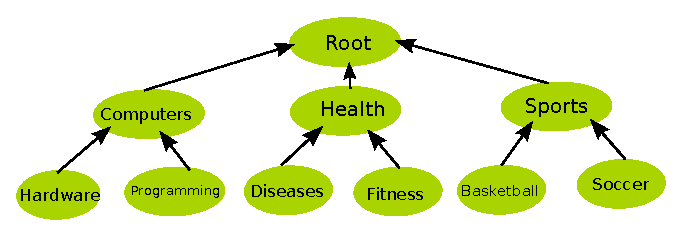
\includegraphics[width=90mm]{cattree}
%\caption{Category tree}
%\label{fig:tree}
%\end{figure}

\subsection{Classification}
To classify the given database we traverse each level of the category tree and compute the following metrics for each category:

\[ECoverage(D,Ci)=\sum_{q \ is \ a \ query \ probe \ for \ C_i}{f(q)} \]

\[ESpecificity(D, C_i ) = \frac{ESpecificity(D, Parent(C_i )) \times ECoverage(D, C_i )} {\sum_{C_j \  is \ a \ child \ of \ Parent(C_i)} {ECoverage(D,C_j)}} \]

pruning the categories that do not meet the specificity and coverage criteria.

\begin{verbatim}
Classify(Ts,Tc)
    Cat={Root}
    insert Root to L
    P=Root
    level=0
    do{
    for each category P in L
        read P query-file  F
        add to L children of P
        for each query q in F
            pose-query(q)
            store top-4 results
            update coverage of P 
            update coverage of q.child
         if(P.specificity>=Ts && P.coverage>=Tc)
            add P to Cat
    }while(levels<=2)
    return Cat
\end{verbatim}

\subsection{Content Summary Construction}

For each category node C (e.g., "Root") that you "visit" while you classify database D (using the Part 1 procedure):

    For each query q associated with this node retrieve the top-4 pages returned by Yahoo! for the query on the database D.


\section{Assumptions}

\begin{itemize}
\item Exception handling
\item Multi-word probes: we decided not include multi-word entries in the content summaries.
\end{itemize}

\section{Example}
To test the classification results of QProber we used the provided the examples in the project description and several of the examples from a list
of Largest Deep Web Sites \cite{AIP}. The following results are for $T_s$=0.6 and coverage $T_c$=100.

\begin{table}
\begin{tabular}{|c|c|c|}
\hline
\textbf{URL} & \textbf{Description} & \textbf{Classification}\\
\hline
java.sun.com & Java@Sun & Root/Computers/Programming \\
\hline
yahoo.com& Yahoo SE& Root\\
\hline
diabetes.org& American Diabetes Asoc.& Root/Health\\
\hline
tomshardware.com & Tom's Hardware &Root/Computers/Hardware\\
\hline
hardwarecentral.com& PC Hardware Reviews & Root/Computers\\
\hline
espn.com & WorldWide Leader in Sports &Root/Sports/Basketball\\
\hline
portal.acm.org & ACM Digital Library &Root/Computer/Programming\\
\hline
hopkins-aids.edu & HIV guide &Root/Health/Diseases \\
\hline
agiweb.org & American Geological Institute & Root/Health \\
\hline
www.cancer.gov & National Cancer Institute& Root/Health/Diseases\\
\hline
www.ncbi.nlm.nih.gov/PubMed & PubMed & Root/Health/Diseases\\
\hline
www.ovid.com/site/index.jsp & Ovid Technologies &Root/Health/Diseases\\
\hline
soccernet.espn.go.com & Football News \& Scores & Root/Sports/Soccer \\
\hline
www.jumbo.com & Free Computer Software & Root/Computers/Programming\\
\hline
www.webmd.com & Medical News \& Information & Root/Health\\
\hline
www.fitnessmagazine.com & Fitness Magazine & Root/Health/Fitness\\
\hline
www.afaa.com & Aerobic \& Fitness Info of America& Root/Health/Fitness\\
\hline
processing.org & Processing Software & Root/Computer/Programming\\
\hline
www.telegraph.co.uk/sport & Telegraph Sport News & Root/Sports/Soccer\\
\hline
nba.com & National Basketball Association & Root/Sports/Basketball\\
\hline
www.sports.org.au & Australian Athletes with Disability & Root/Sports\\
\hline
\end{tabular}
\label{}
\end{table}

\section* {Appendix}

\subsection* {File Listing}

We list below the files included in out submission zip. The zip contains the following folders:

[src, lib, queries].
The files are:
\begin{itemize}
\item README.pdf
\item src/YahooProber.java
\item src/URLProcessor.java
\item src/Makefile
\item lib/json.jar
\item queries/Root.txt
\item queries/Computers.txt
\item queries/Health.txt
\item queries/Sports.txt
\end{itemize}

\subsection* {Compilation}
\begin{itemize}
\item \textbf{Compile}: make 
\item \textbf{Clean-up}: make clean 
\item\textbf{Execute}: java -cp .:../lib/json.jar  YahooProber $<url>$ $<t_{es}>$ $<t_{ep}>$ $<yahoo-app-id>$
\item \textbf{Yahoo App Id}: 

BEWTNqTV34H1zojJNQ5MZB48A1vR2mJeNAhKRvk5.bLyZd6gYgQmsVVsqZ7vv32aW73O6VNyzTO
\end{itemize}


\begin{thebibliography}{50}
		\bibitem{AIP} \textit{Largest Deep Web Sites}, \url{http://aip.completeplanet.com/aip-engines/help/largest_engines.jsp}
		\bibitem{QProb} \textit{QProber: A system for automatic classification of hidden-web databases}, Panagiotis G. Ipeirotis,  Luis Gravano,  Mehran Sahami, 2003
\end{thebibliography}

\end{document}